\documentclass{standalone}
\usepackage{tikz}
\usetikzlibrary{arrows.meta}
\tikzset{>={Latex[width=3mm,length=3mm]}}
\definecolor{Color1}{RGB}{255,0,0}
\definecolor{Color2}{RGB}{255,165,0}
\definecolor{Color3}{RGB}{0,255,0}
\begin{document}
	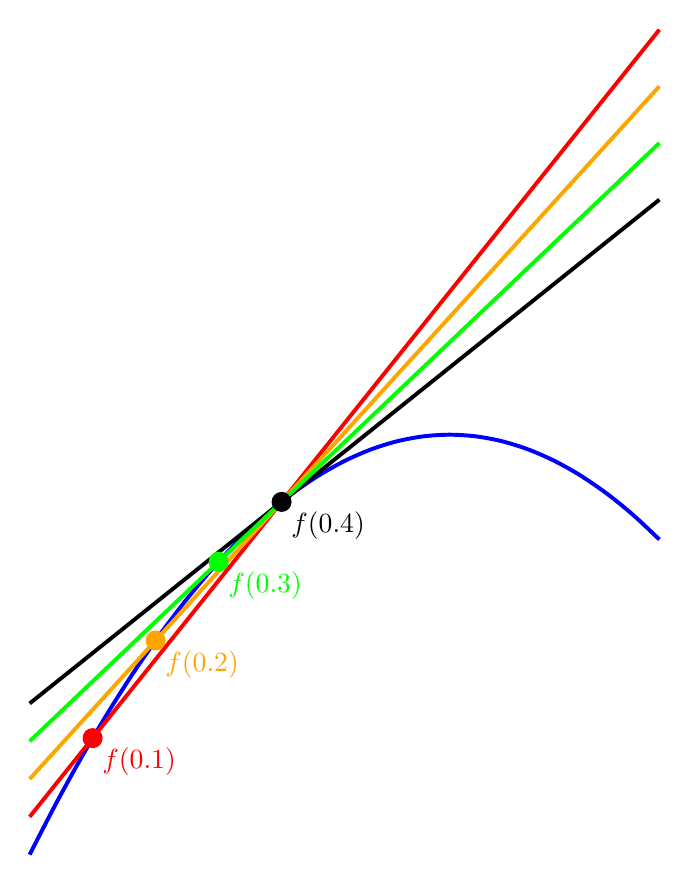
\begin{tikzpicture}[scale=4,x=2cm,y=2cm]
		% curve
		\draw[scale=1,domain=0:1,blue,smooth,variable=\x,line width=0.5mm] plot ({\x},{2.0*(1-\x)*\x + 0.5*\x*\x});	

		% actual slope
		\draw[scale=1,domain=0:1,black,smooth,variable=\x,line width=0.5mm] plot ({\x},{0.8*\x+0.24});		

		% approximated slopes
		\draw[scale=1,domain=0:1,Color1,smooth,variable=\x,line width=0.5mm] plot ({\x},{1.25*\x+.06});			
		\draw[scale=1,domain=0:1,Color2,smooth,variable=\x,line width=0.5mm] plot ({\x},{1.1*\x+.12});		
		\draw[scale=1,domain=0:1,Color3,smooth,variable=\x,line width=0.5mm] plot ({\x},{0.95*\x+.18});	

		% f(0.4) dot and label
		\draw[black,fill=black] (0.4,0.56) circle (0.015);	
		\draw[black]    (0.4,0.56) node[anchor=north west] {$f(0.4)$};

		% f(0.1) dot and label
		\draw[Color1,fill=Color1] (0.1,0.185) circle (0.015);	
		\draw[Color1]    (0.1,0.185) node[anchor=north west] {$f(0.1)$};				

		% f(0.2) dot and label
		\draw[Color2,fill=Color2] (0.2,0.34) circle (0.015);	
		\draw[Color2]    (0.2,0.34) node[anchor=north west] {$f(0.2)$};		

		% f(0.3) dot and label
		\draw[Color3,fill=Color3] (0.3,0.465) circle (0.015);	
		\draw[Color3]    (0.3,0.465) node[anchor=north west] {$f(0.3)$};		

	\end{tikzpicture}
\end{document}

% A*s^2    0
% B*2*s*t  1
% C*t^2    0.5
% f(x) = 2*(1-x)x + 0.5*x*x
% f(0.4) = 2*0.6*0.4 + 0.5*0.4*0.4 = 0.56

% f(0.1) = 2*0.9*0.1 + 0.5*0.1*0.1 = 0.185
% f(0.2) = 2*0.8*0.2 + 0.5*0.2*0.2 = 0.34
% f(0.3) = 2*0.7*0.3 + 0.5*0.3*0.3 = 0.465
% f(0.5) = 2*0.5*0.5 + 0.5*0.5*0.5 = 0.625
% f(0.6) = 2*0.4*0.6 + 0.5*0.6*0.6 = 0.66

% f'(x) = 2 * (1-x + -0.5*x)
% f'(0.4) =  2 * ((1-0.4)+(-0.5*0.4)) = 0.8
% y = mx + b
% y = 0.8*x+0

% A*s^3      : 0.8 -> 0.9  -> 1.0
% B*3*s^2*t  : 1   -> 0.8 - > 0.6
% C*3*s*t^2  : 0.9 -> 0.8  -> 0.7
% D*t^3      : 1   -> 0.9  -> 0.8